\section{Experiments}
\label{sec:experiments}
We run all experiments on a high-performance computing cluster with dual AMD EPYC 9654 processors, 192 CPU cores, and 768GB RAM, using 10–32 cores per run.
\subsection{Experiments with Line and Torus Mappers}
\label{ssec:line_torus_sec}

\begin{figure}
    \centering
    
\includegraphics[width=0.45\linewidth, align = c]{line_torus.png}
    
\includegraphics[width=0.54\linewidth, align= c]{loss_vs_n.pdf}
    \caption{(Left) Examples of line and torus mappers, the latter featuring a loop of height 11. (Right) The loss function and resulting upper bound computed for this pair of graphs over varying values of $n$. In both figures, letters denote critical vertices and numbers denote regular vertices.}
    \label{fig:loss_vs_n}
\end{figure}

We validate our loss-function optimization by testing it on two simple mapper graphs whose interleaving distances can be computed by hand. 
The first is the \emph{line mapper graph} $L$, consisting of a single vertex at each integer function value and edges connecting sequential vertices. 
The second is the \emph{torus mapper} $T_h$, which is a mapper graph of a height function on an upright torus and contains a loop of height $h$.
%
Both mappers are defined over the same range of function values; see the left panel of \cref{fig:loss_vs_n} for an example with $h = 11$. 
It is straightforward to verify that 
%
$d_I(L, T_h) = \lceil h/4 \rceil$; for $h = 11$, this gives $d_I(L, T_{11}) = 3$. 

\subsubsection{Loss Optimization vs Theoretical Computations}

We compare the results of the ILP with the hand-computed interleaving distance on the line and torus mappers. In the right panel of \cref{fig:loss_vs_n}, we see that the loss computed for varying choices of $n$ achieves the true interleaving distance for all $n$ up to and including the actual interleaving value. 
Thus, in this particular example, a search over $n$ would not be required. However, this behavior cannot be assumed \textit{a priori}; see \cref{ex:binarySearchExample} for a case where the search is indeed necessary.
Note that we obtain the interleaving maps as a byproduct of this computation, see \cref{fig:optimizedmap} for an example of the output optimal interleavings.
%
We compute the distances across varying loop height ($h$).
%
For each mapper pair, we perform 50 iterations of loss optimization and in every case the ILP returns the optimal solution with the same optimized loss value, empirically demonstrating the stability of our optimization pipeline. 
%
%
%
%
%
%
%
%
%

\begin{figure}
\centering
        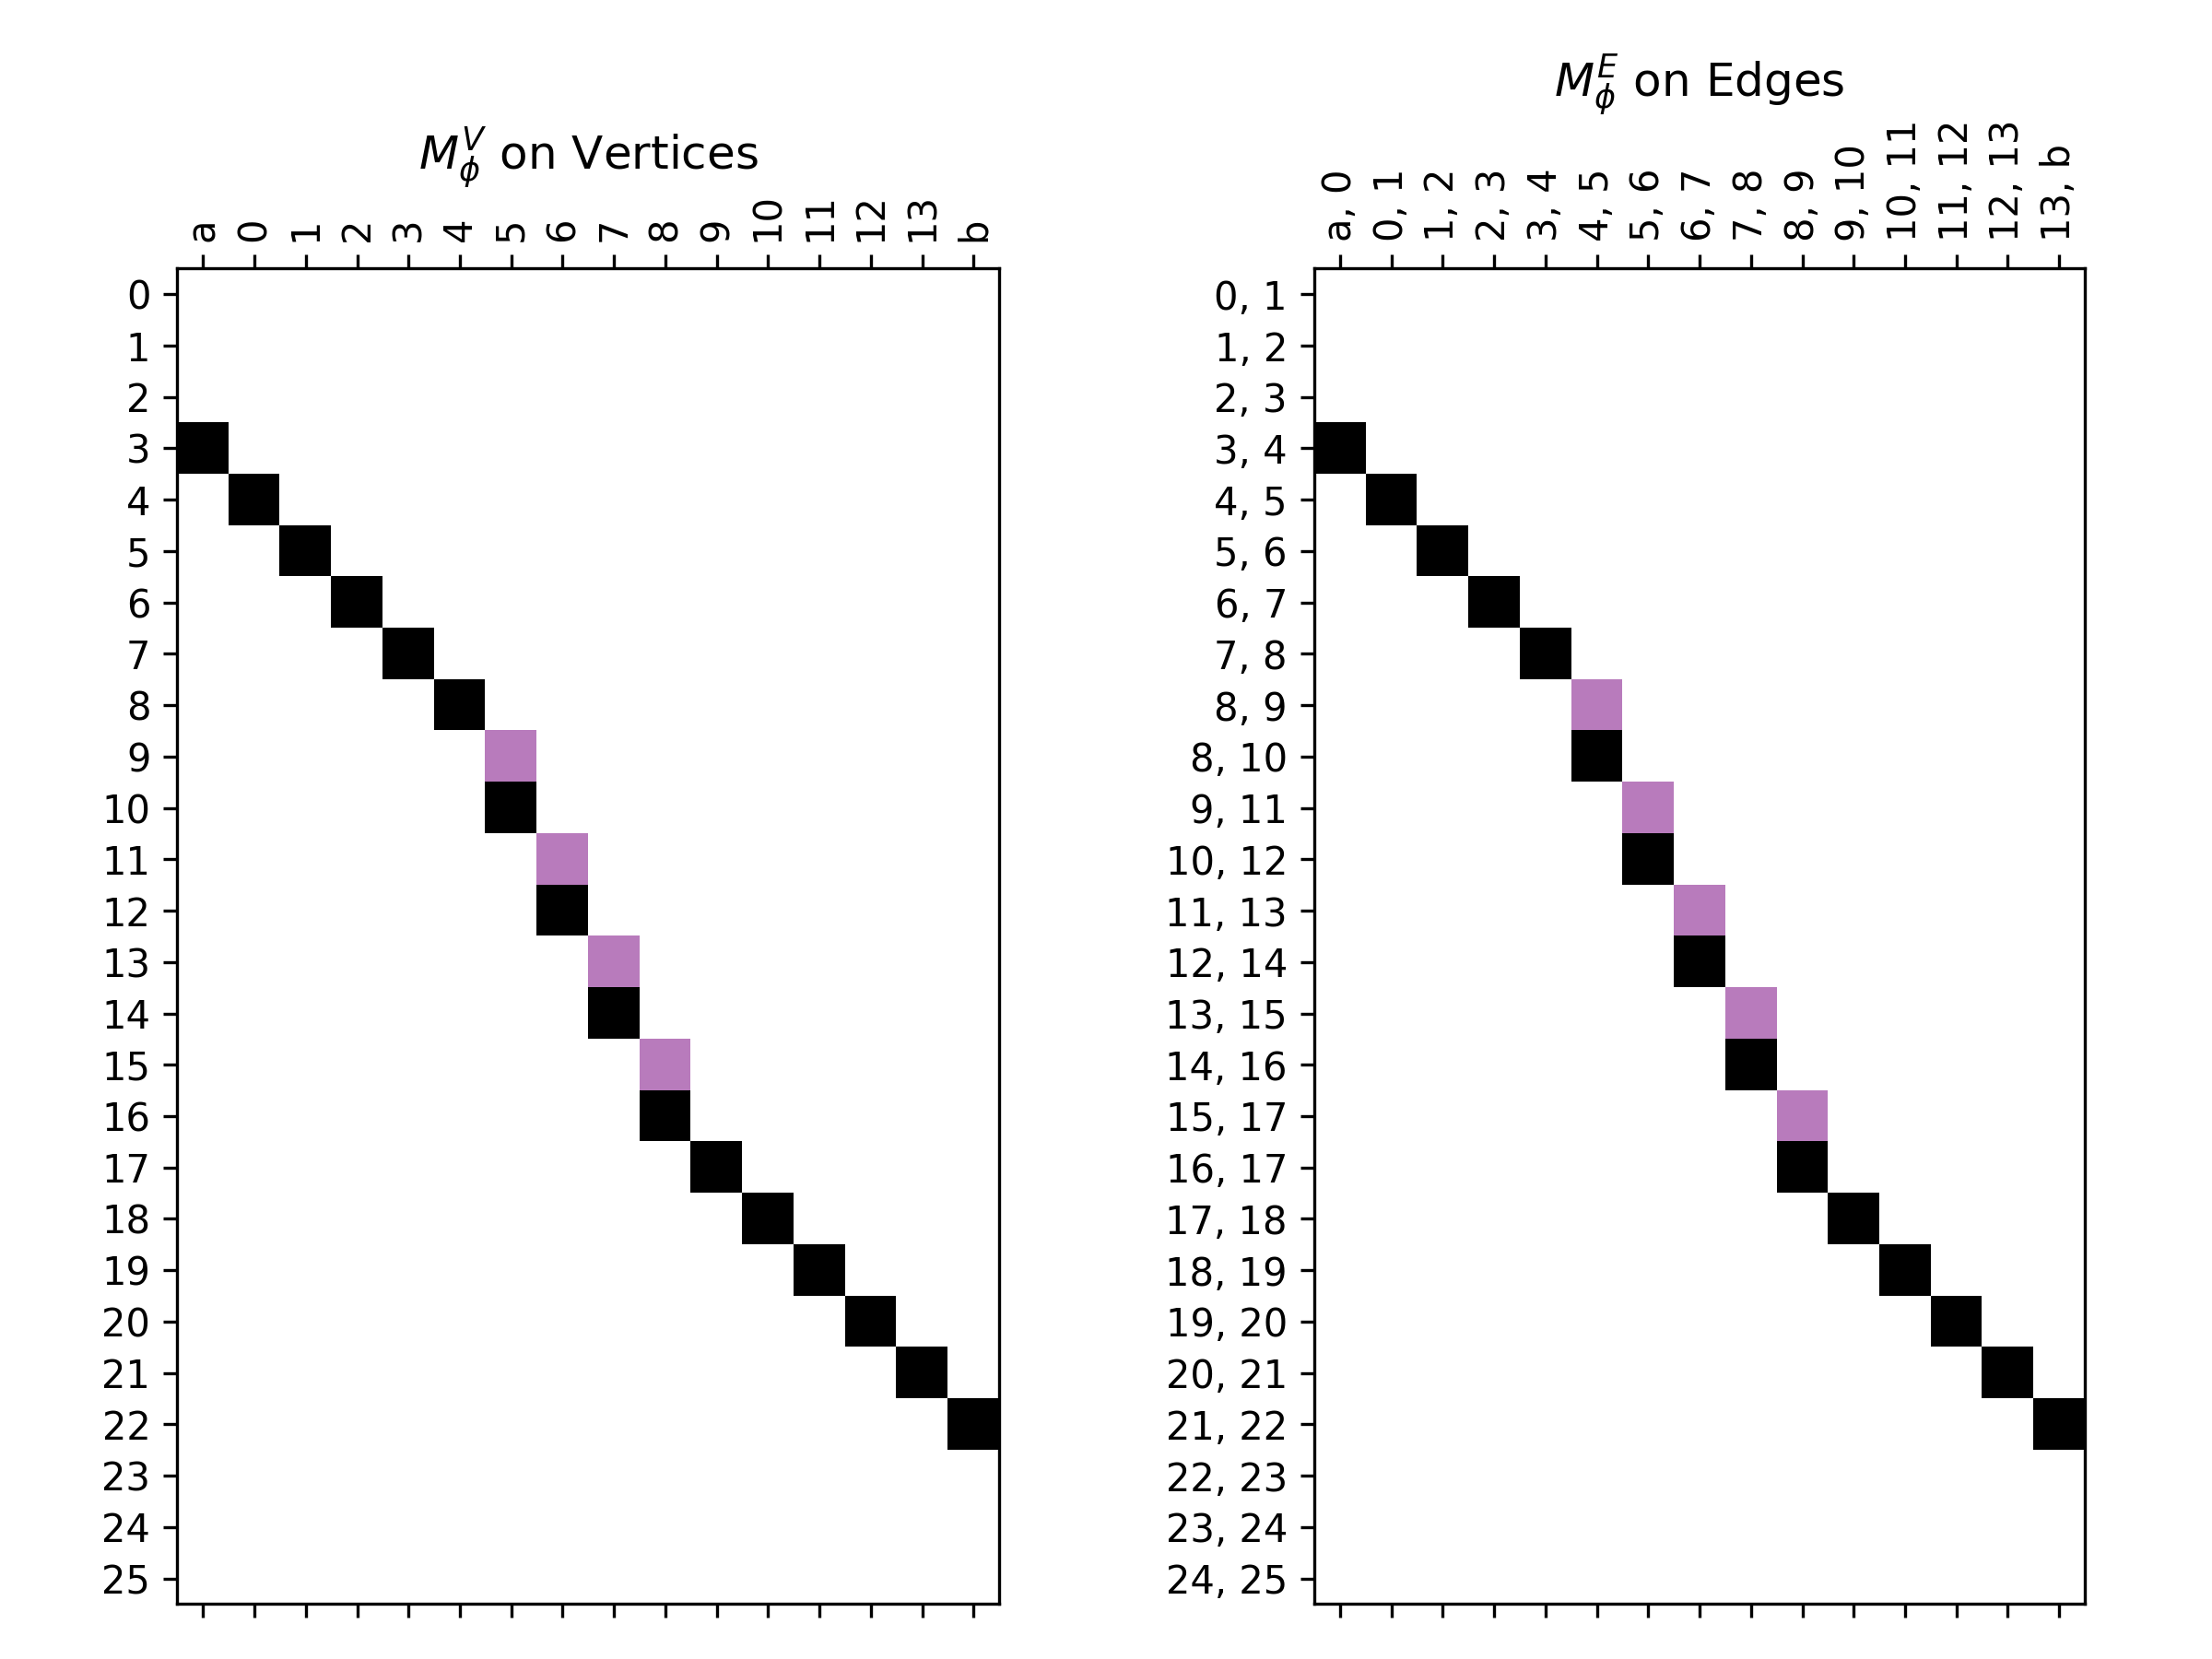
\includegraphics[width=.8\linewidth, align = c]{figures/torus_line_optimized_maps.png}
        
\includegraphics[width = .07\textwidth, align = c]{colorbar-PurBl-binary.png}
\caption{The optimized map from the line mapper to the 1-smoothed torus from the example in \cref{fig:loss_vs_n} (left)).}
\label{fig:optimizedmap}
\end{figure}

%
%

 %

 %

%
%
%
%
%
%
%
%
%
%
%
%
%
%
%
%
%

\subsubsection{Comparing Loss Optimization with \cref{prob:BinaryDecision} and \cref{prob:LossComputation}}
\label{ssec: p2_p3_benchmark}
By \cref{cor:p2_p3_equiv}, the optimization problems \cref{prob:BinaryDecision} and 
\cref{prob:LossComputation} are equivalent and either may be used 
to compute an upper bound on the interleaving distance.
We compare the runtime of \cref{prob:BinaryDecision} and \cref{prob:LossComputation} on the same torus and line mapper pairs described above, varying the loop height $(h)$. 
For each $h$, we measure both the total runtime, which includes both pre-computing the necessary matrices and the ILP optimization, and the ILP optimization time alone, averaged over 10 repetitions.

\begin{figure}
    \centering
    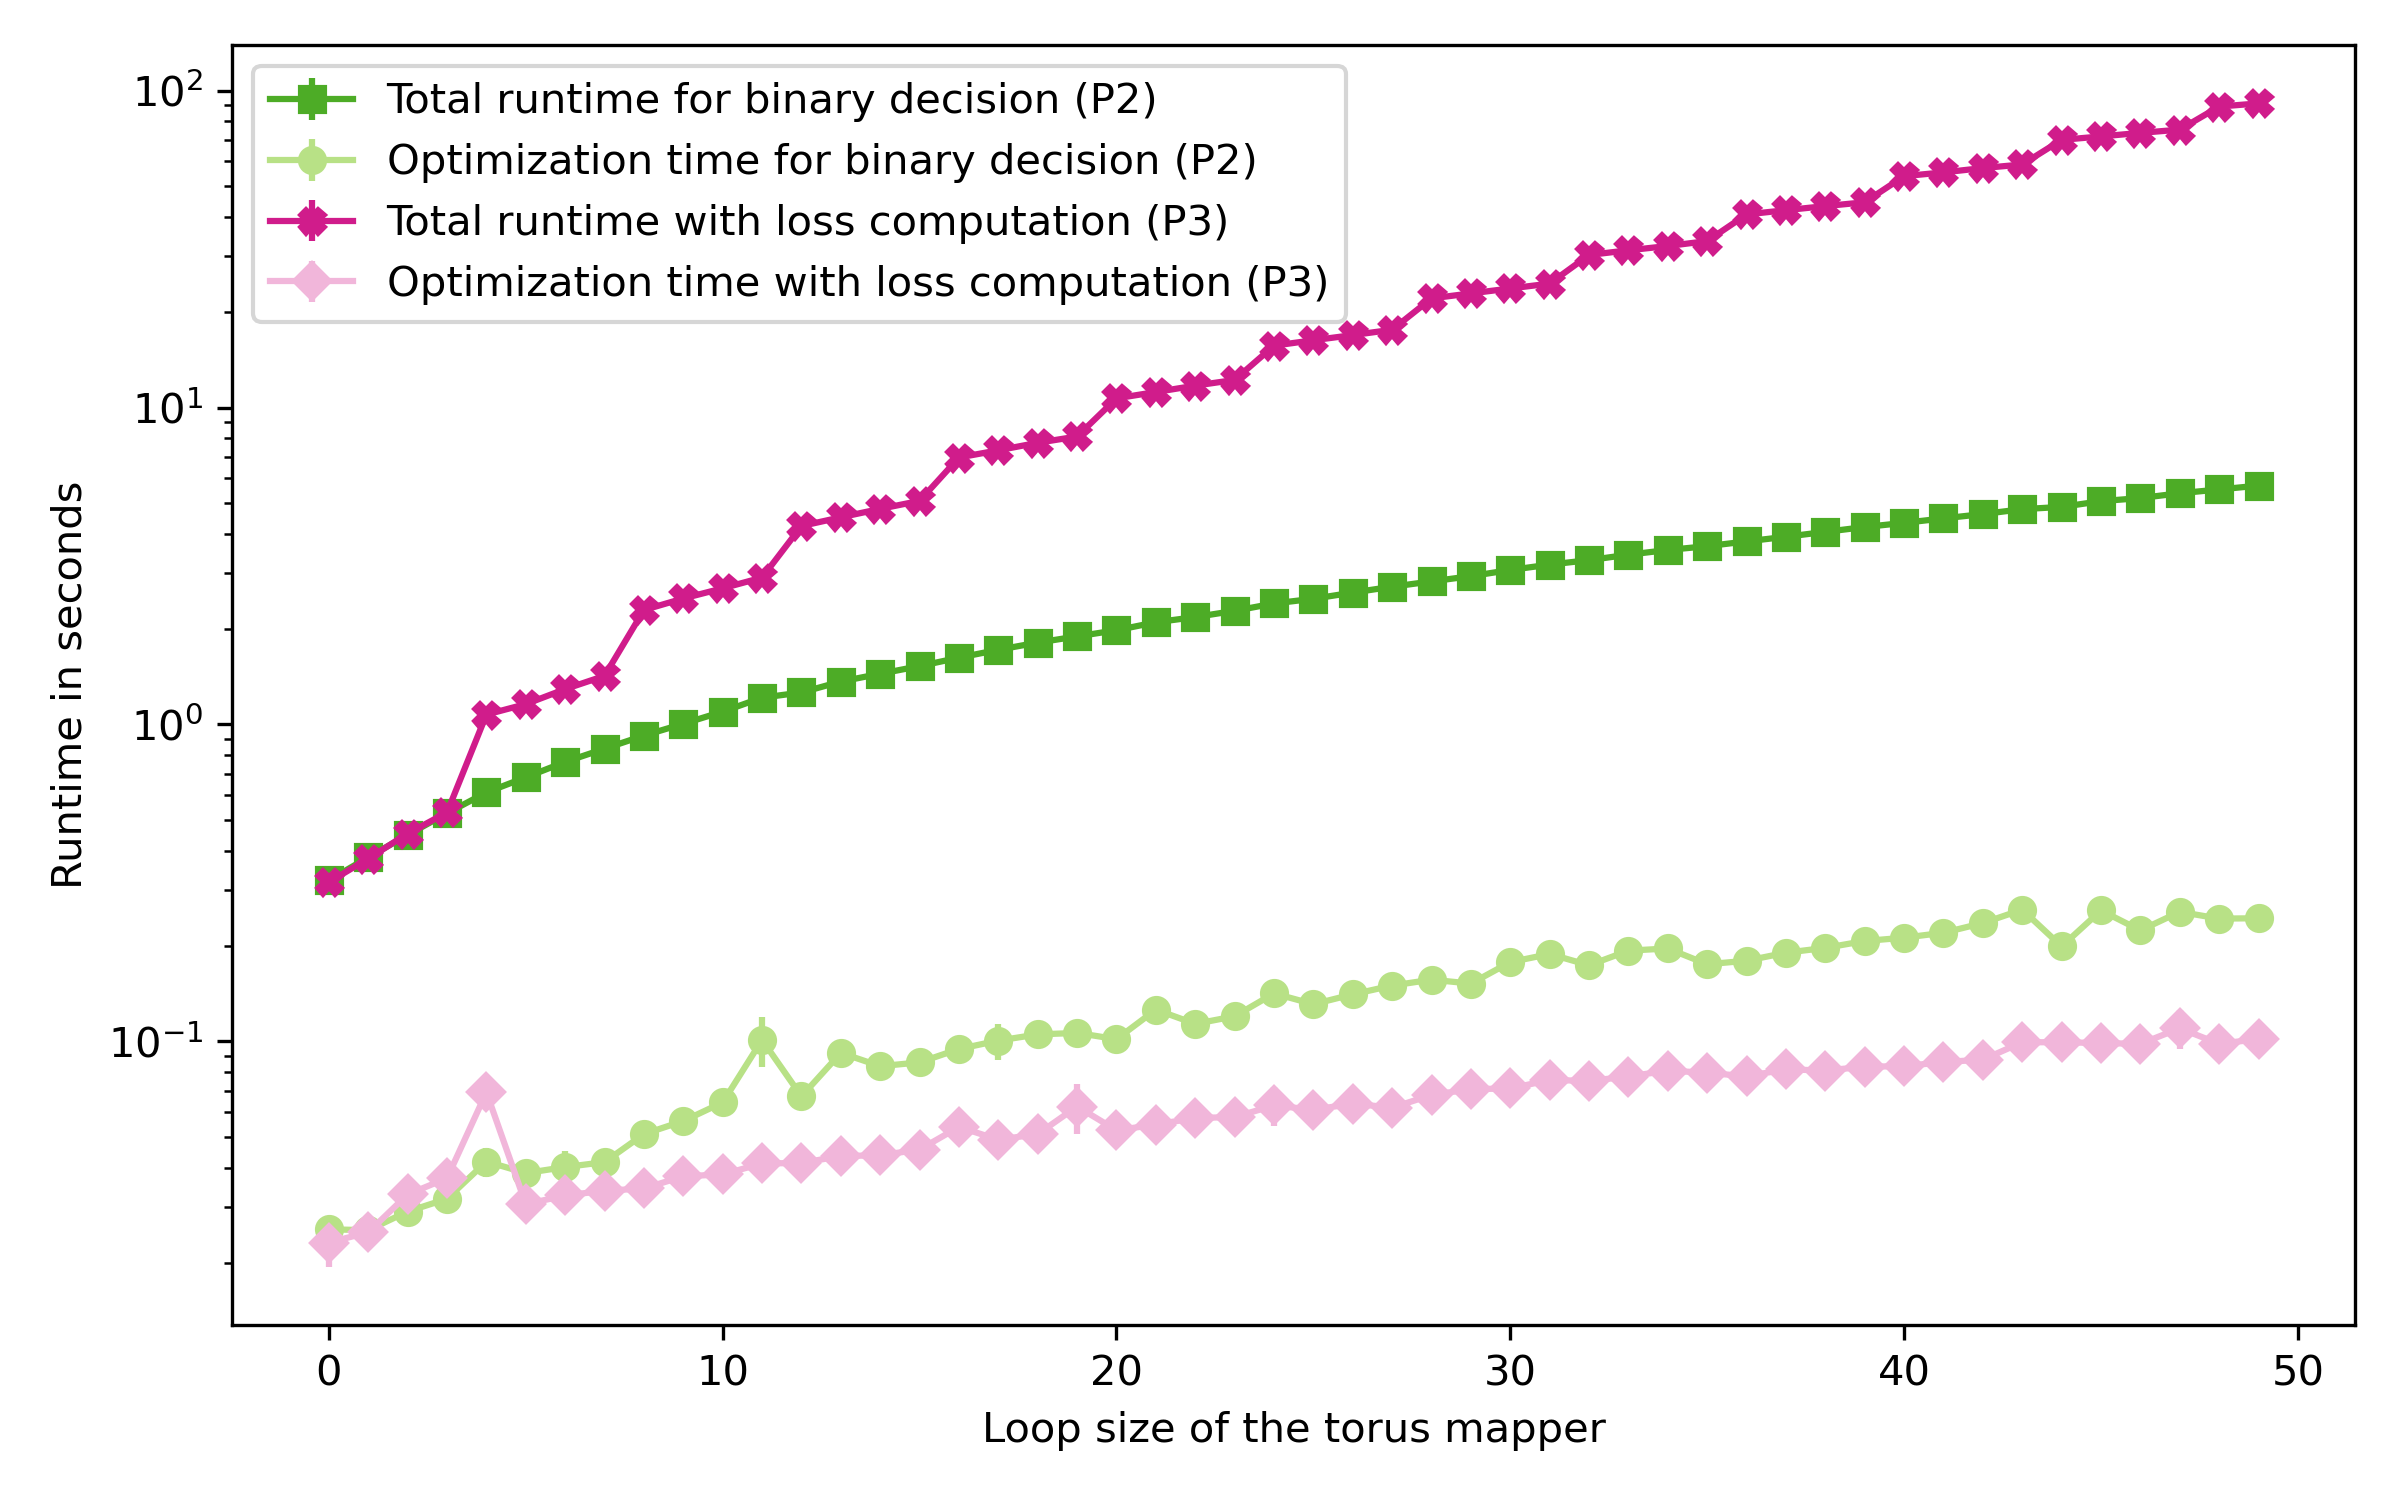
\includegraphics[width=0.7\linewidth]{figures/torus_line_benchmark.png}
    \caption{Total and ILP optimization runtime (log scale) for \cref{prob:BinaryDecision} (binary decision, green) and \cref{prob:LossComputation} (loss computation, pink), varying the loop height $h$ of the torus mapper, averaged over 10 repetitions. The additional overhead in \cref{prob:LossComputation} is due to the pre-computation of the distance matrix D.}
    \label{fig:p2_p3_benchmark}
\end{figure}

As shown in \cref{fig:p2_p3_benchmark}, \cref{prob:BinaryDecision} is consistently faster than \cref{prob:LossComputation} in total runtime, except for very small mappers, where there's no difference in runtime. 
However, as the mappers grow in size, the gap in runtime widens. 
On the other hand, when we compare ILP optimization time alone, \cref{prob:LossComputation} is marginally faster than \cref{prob:BinaryDecision}.
This suggests that the overhead in \cref{prob:LossComputation} mostly comes from the pre-processing cost of computing the distance matrix $D$, which requires performing shortest-path computations on the thickened graph for each function value block at every iteration.

We attribute the slightly faster ILP solve time in \cref{prob:LossComputation} to the difference in the problem formulation.
\cref{prob:BinaryDecision} is a pure feasibility problem with hard equality constraints, which demands the solver to certify infeasibility when no solution exists.
\cref{prob:LossComputation}, in contrast, tries to minimize the loss function, which always has a finite solution.
In all experiments, both \cref{prob:BinaryDecision} and 
\cref{prob:LossComputation} return the same interleaving distance 
bound, consistent with \cref{cor:p2_p3_equiv}.
These results suggest that while the two formulations are theoretically equivalent, \cref{prob:BinaryDecision} is currently preferable in practice when computational efficiency is the priority.

\subsection{Classification Experiments}
\label{ssec:ClassificationBrief}
%

We ran two proof-of-concept classification experiments using this optimized loss on the mapper interleaving distance. 
The details are provided as follows.
\subsubsection{Classification of Binary Images}
\label{ssec:ClassificationMPEG7}
%

We conducted a classification experiment on the MPEG-7 dataset \cite{jeannin1999}, specifically MPEG-7 CE
Shape-1 Part B, which is a widely used benchmark for shape analysis and classification with binary
images.
The results are shown in \cref{fig:image_mds}.
Our methodology involves computing mapper graphs from the dataset and analyzing their interleaving distance for classification tasks.

In this experiment, we choose six image classes, \emph{apples, cups, forks, hearts, horseshoes} and \emph{sea snakes}, and select 10 images from each class.
See \cref{fig:image_mds}  (left) for examples in each category.
We convert these images to mapper graphs using {\it KeplerMapper} \cite{van2019kepler}, where the lens function is given by the $y$-coordinate of each pixel. For every point cloud, we use a cover of 10 elements with a $30\%$ overlap, and set the epsilon value for DBSCAN to 3. These parameters are chosen to generate a mapper graph which best represents the input image.
For each resulting mapper graph, we choose parameter values to ensure that there is only one connected component in the graph.
For each node, we assign the function value, or \emph{height}, of that node to be the midpoint of the cover element it belongs to, and normalize so that all node heights are in the range $[0, 20]$. 
This normalization ensures consistency in mapper size, simplifying loss computation.


Once the mapper graphs are obtained, we compute the optimal upper bound of the interleaving distance between them using the optimization strategy discussed earlier, which serves as a measure of similarity between mapper graphs. 
To visualize the distance performance, we construct a {\it multi-dimensional scaling} (MDS) \cite{borg2007modern} plot (\cref{fig:image_mds}, right) using the computed distance matrix (MDS stress is 0.14, which ensures good goodness-of-fit). 
MDS is chosen for visualization as it accepts an arbitrary distance matrix as input. 

As we see in \cref{fig:image_mds} (right), the optimal upper bounds on distance successfully cluster similar shapes together. 
This behavior reflects what the interleaving distance is designed to capture: the distance is small only when mapper graphs agree in both graph structure \emph{and} lens function. 
Among all categories, {\it apple} exhibits the most well-defined grouping. 
Additionally, some of the other shapes are well separated, such as {\it apple} and {\it fork} or {\it seasnake}.
However, certain shapes are not differentiated by this distance. 
For instance, the {\it cup} category in the MPEG-7 dataset includes two types of cups: one with joined handles, forming a loop, and another without joined handles. 
This structural difference is reflected in the mapper representation, causing a few to appear far apart despite belonging to the same category.  
This is to be expected since the mapper interleaving distance is built to find similar topological structure in the resulting graph, and does not take the geometric similarity into account. 
Likewise, the horseshoes and sea snakes, despite being similar structurally, have a large distance between them since the mapper graph lens function takes the embedding direction into account; the horseshoe with opening of the U-shape pointing down and the sea-snake with the opening point up are considered very different under this distance. 

We also use the pairwise distances to classify the images into their correct classes using $k$-nearest neighbors ($k$-NN) \cite{cover1967nearest}, based on the optimized loss computed on the mappers.
To determine the optimal number of neighbors $(k)$ and avoid overfitting or underfitting, we first perform a $5$-fold cross-validation on the data, testing values of $k$ from $1$ to $30$.
The optimal $k$ was selected to be $1$, which resulted in the highest and most stable accuracy of $91.67\%$, as shown in \cref{fig:image_knn} (left).
\begin{figure}
    \centering
    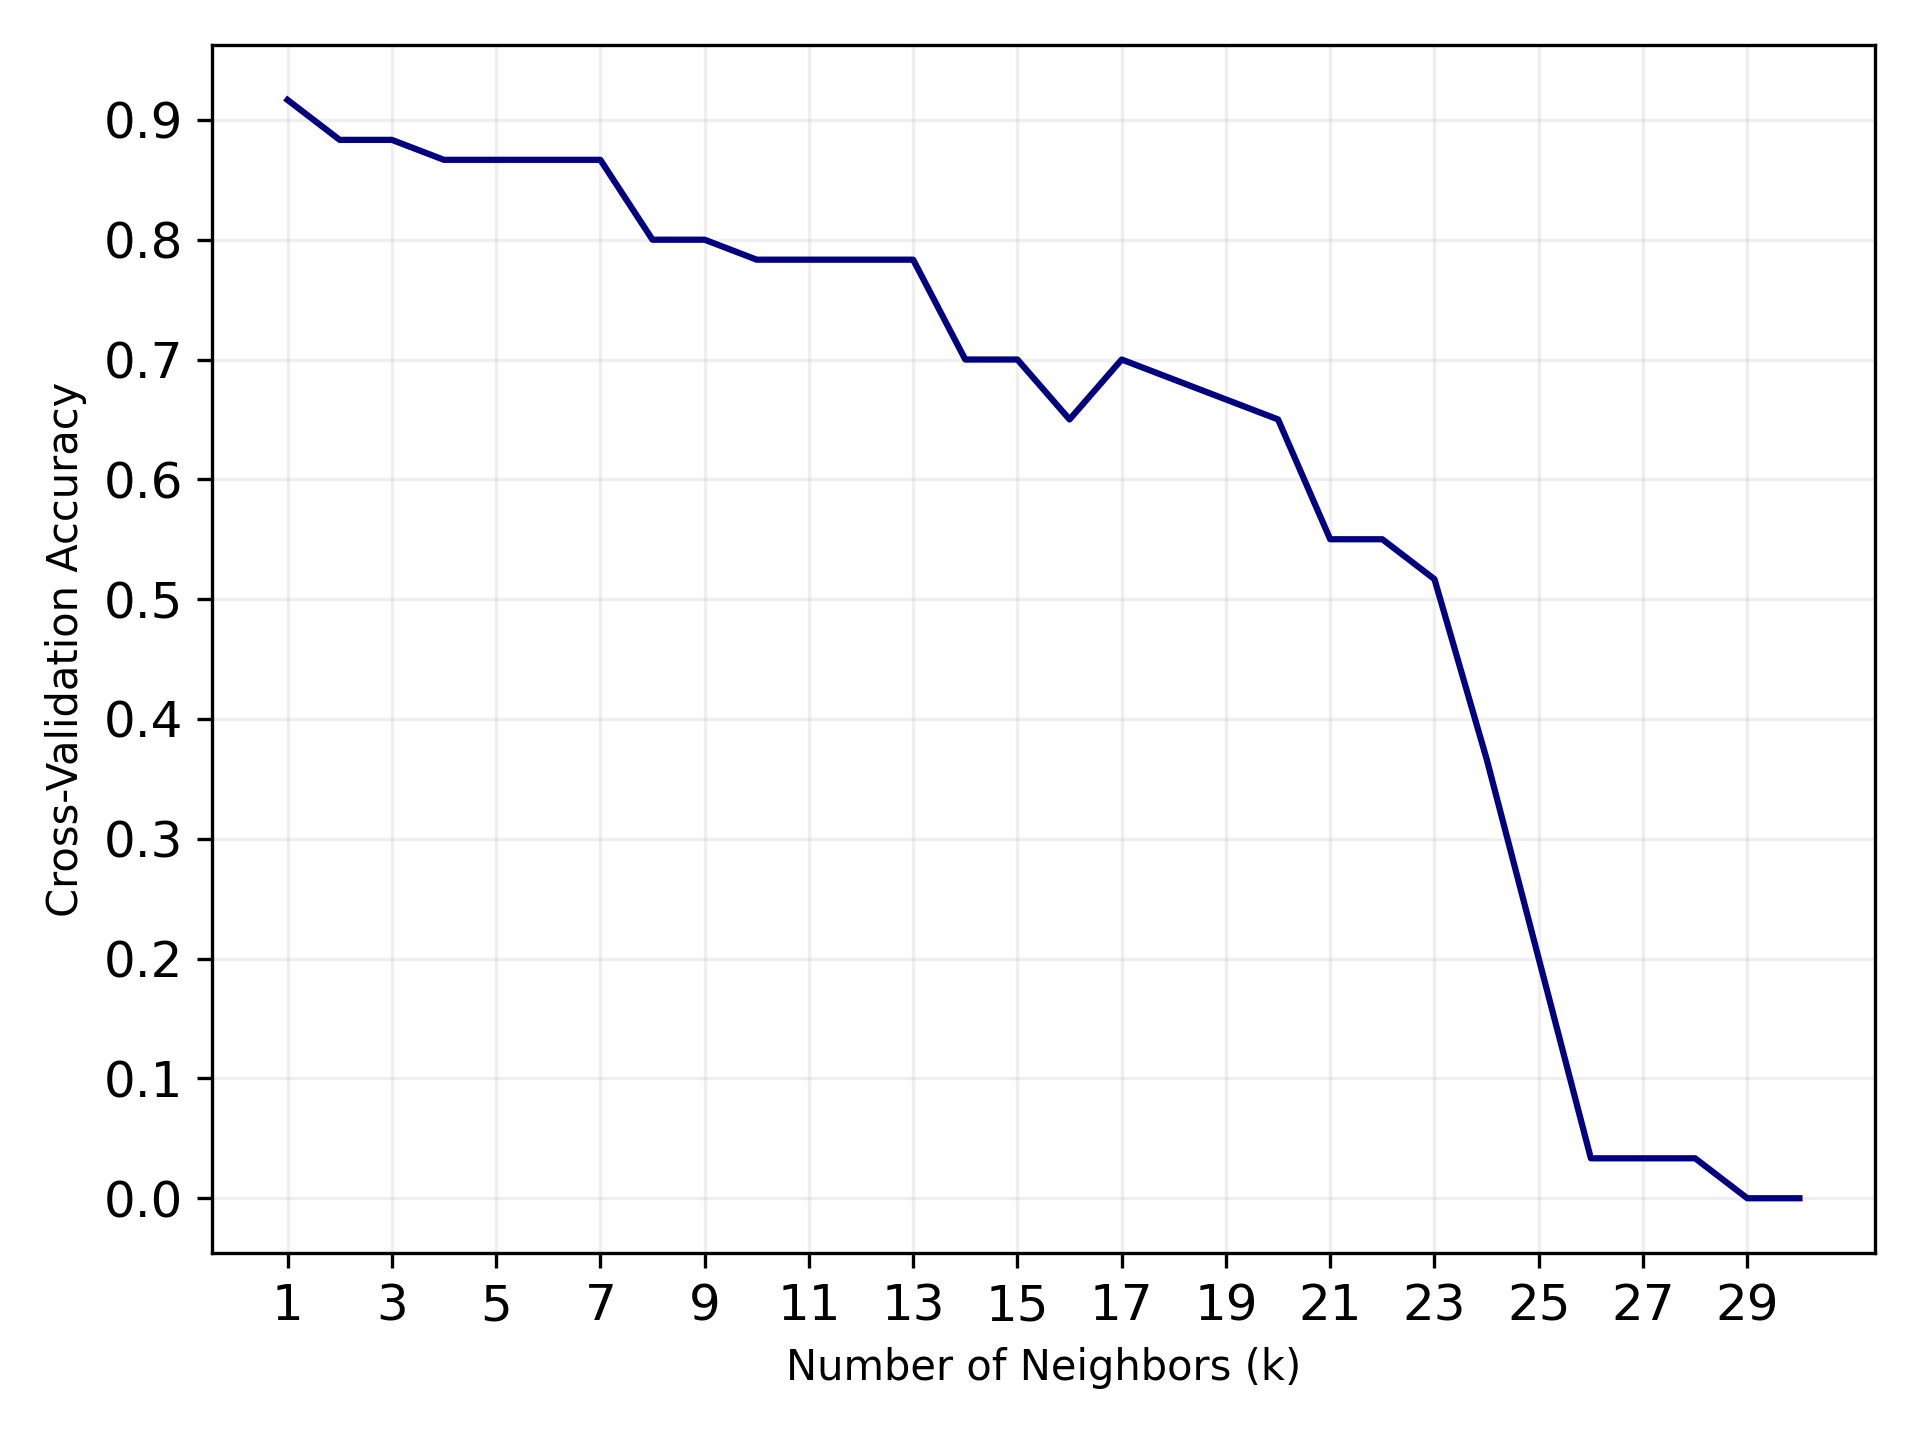
\includegraphics[width=0.46\textwidth]{figures/knn_accuracy_vs_k.png}
    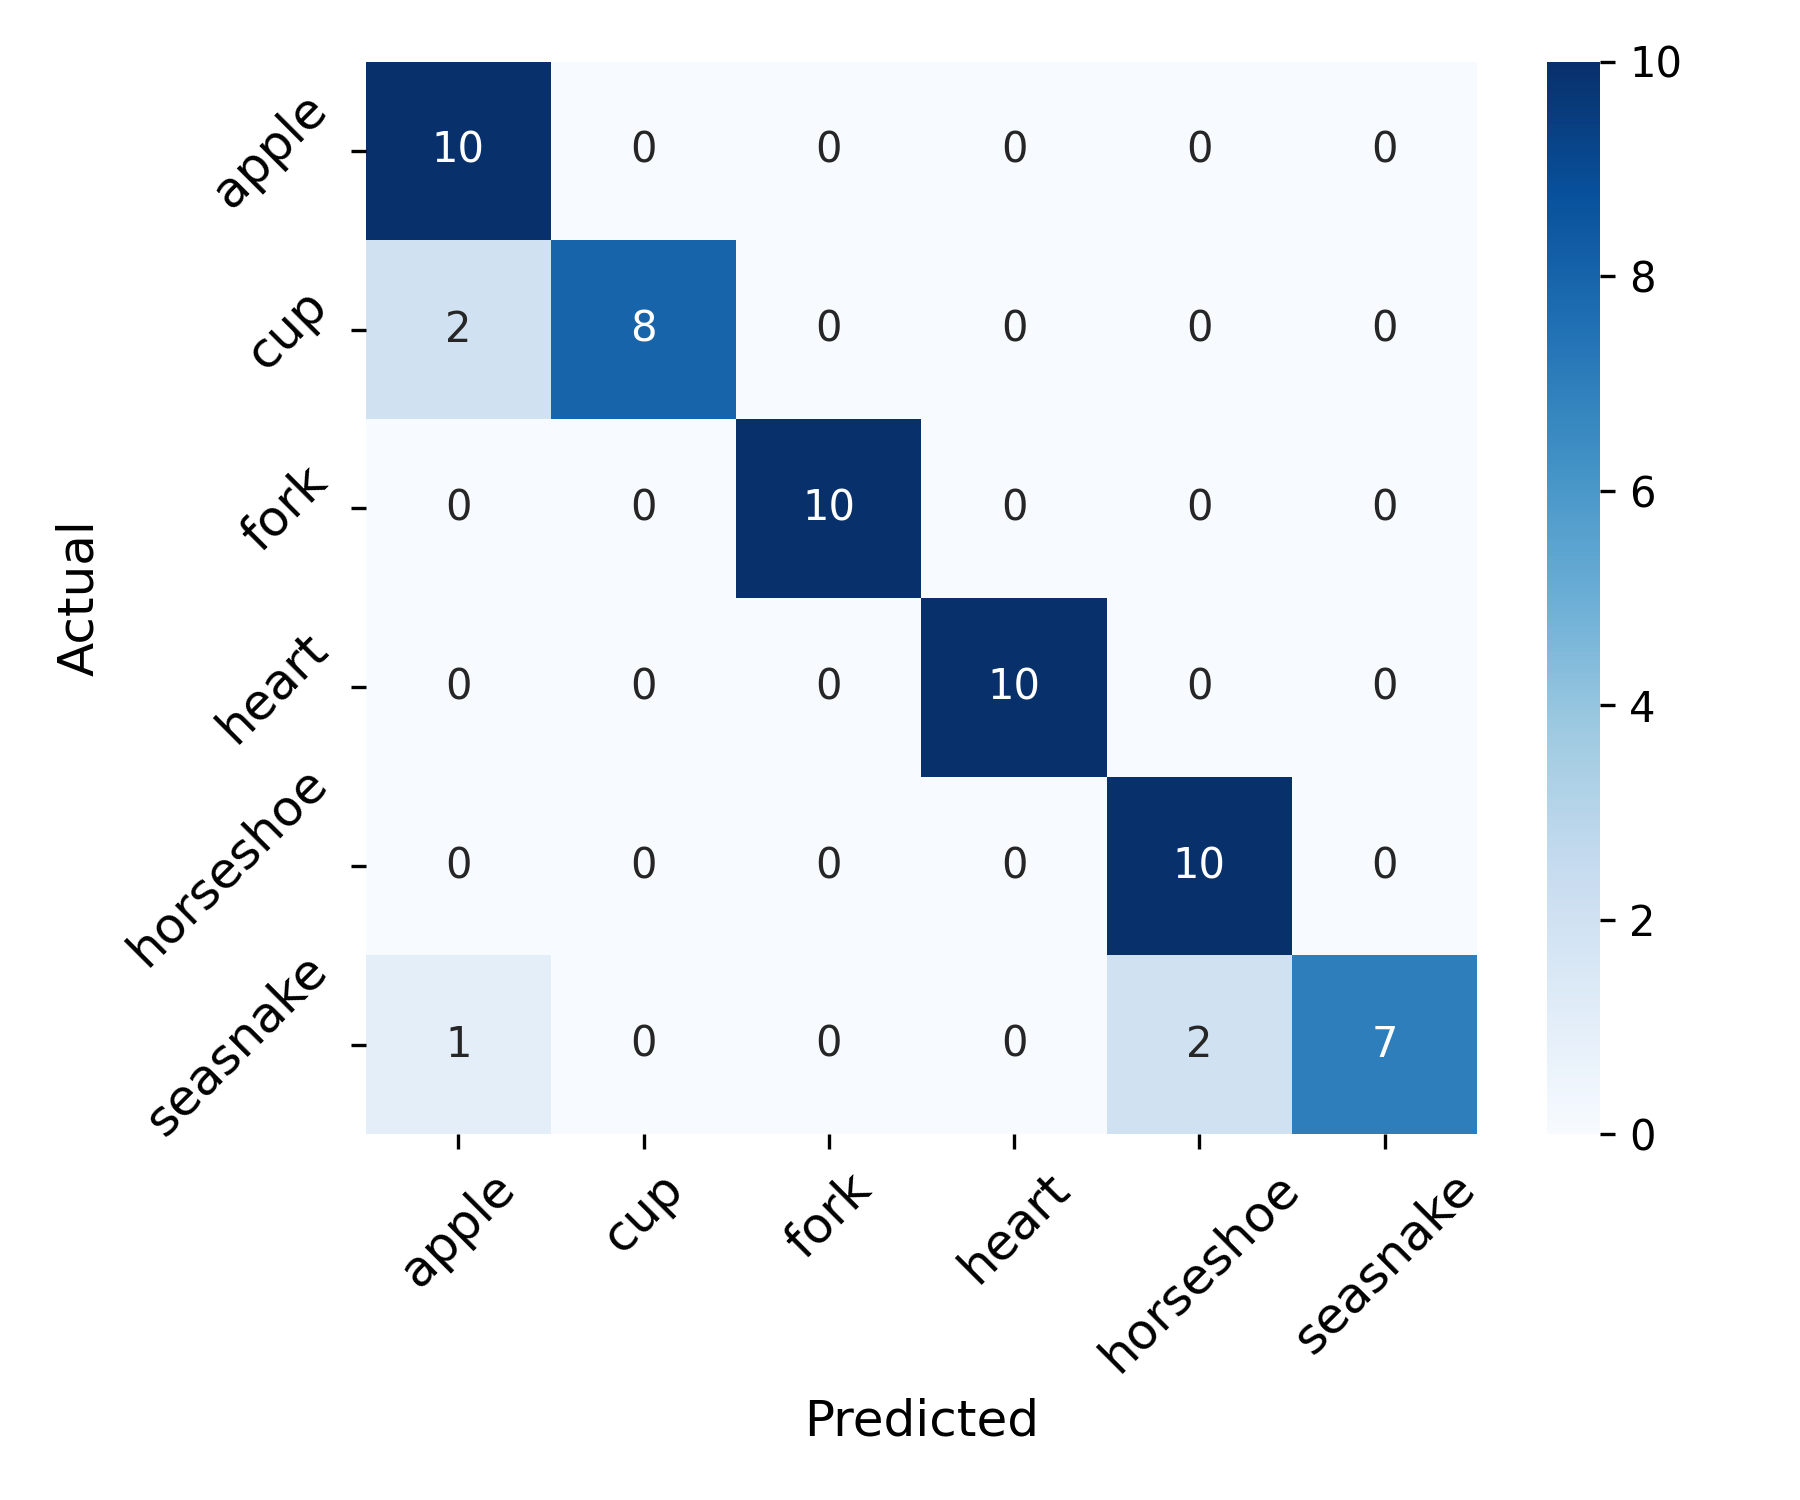
\includegraphics[width=0.45\textwidth]{figures/confusion_matrix.png}
    \caption{(Left) Accuracy of KNN classifier for different $k$ values during 5-fold cross-validation. The optimal $k = 1$ achieved $91.67\%$ accuracy.\\
    (Right) Confusion matrix showing how the actual classes match with the predicted class. Each $(i,j)$-th cell indicate number of times an image from category $i$ was classified as category $j$.}
    \label{fig:image_knn}
\end{figure}
For a more robust evaluation, we also implement {\it leave-one-out cross-validation} (LOO-CV), where one data point is used as a test case while the rest are used for training the model.
To visualize the classification and misclassification, we display a {\it confusion matrix}, which highlights the categories that are being misclassified, see \cref{fig:image_knn} (right).
The LOO-CV results confirm the model's accuracy of $91.67\%$, indicating that while the model is generally effective, there are still some misclassifications.
It is important to note that this is a preliminary experiment with only 10 images per category (totaling 60 images), and expanding to the full MPEG-7 dataset might improve accuracy.
As we see in the confusion matrix in \cref{fig:image_knn} (right), the categories that suffer from misclassification are {\it cup} and {\it seasnake}. 
As discussed before, the some of the cups have joined handles and some do not, which contributes to the misclassification.
Additionally, the sea snake images are highly varied in how they are oriented, leading to misclassification due to differences in their embeddings, which results in generation of very different mapper graphs.


 %
%
%
%
%
These results suggest that the computed distance bound indeed captures meaningful topological differences in the data, indicating its potential usefulness in further real-world applications.



\begin{figure}
    \centering
    
\includegraphics[width=0.42\linewidth, align = c]{point_clouds.png}
    
\includegraphics[width=0.52\linewidth, align = c]{mds_plot.png}
    \caption{(Left) Example images for six categories of images from the MPEG-7 dataset.
    (Right) MDS plot computed on the pairwise optimal upper bound for the interleaving distance.}
    \label{fig:image_mds}
\end{figure}

\subsubsection{Classification of Alphabet Letters}
\label{ssec:ClassificationLetters}

Alongside the binary images, we also conduct a classification experiment on synthetically generated point clouds of six English letters: \textit{A, B, D, I, M, R}.

For each letter, we generate nine 2D point clouds by varying the number of points (500, 700, 1000) and adding Gaussian noise with standard deviation (0, 0.01, 0.02). 
The point clouds are created using geometric representations of each letter.
Different sampling densities and added noise are meant to mimic real-world variability.
\cref{fig:mds_letters} (left) demonstrates how varying the number of points and noise affects the letter \textit{A}.
We follow the same classification pipeline as used for the binary images in \cref{ssec:ClassificationMPEG7}.
Each point cloud is converted into a mapper graph using \textit{KeplerMapper} \cite{van2019kepler}, with the $y$-coordinate of each point as the lens function.
We choose parameter values so that each mapper has a single connected component, and for each node we assign the function value, or \emph{height}, to be the midpoint of the cover element it belongs to, normalized so that all node heights lie in the range $[0, 20]$.
For every mapper, we use a cover of 10 elements with $30\%$ overlap, with DBSCAN (eps=3) as the clustering algorithm.
These parameters were found to best capture the structure of the data.

\begin{figure}[h]
    \centering
    
\includegraphics[width=0.45\linewidth, align = c]{letters_with_noise.png}
    
\includegraphics[width=0.5\linewidth, align= c]{mds_interleaving_alphabet.png}
    \caption{(Left) Point clouds generated for the letter \textit{A} with varying sample density and noise.
    (Right) MDS plot computed on the pairwise optimal upper bound for the interleaving distance.}
    \label{fig:mds_letters}
\end{figure}

We then compute the pairwise optimal upper bound of the interleaving distance and use this as a similarity metric for classification.
To visualize the clustering of different letters, we construct an MDS plot, shown in \cref{fig:image_mds} (right).
The results demonstrate that letters with distinctive shapes, such as \textit{A} and \textit{W}, form clear clusters.
However, some letters such as \textit{R} struggle to cluster distinctly, and distances between certain letters, such as between samples of \textit{R} and \textit{B}, can be small.
This is expected, given the similarity in their mapper graph structures, especially when point density is low and noise is high.

We run a classification task using the pairwise similarity metric to classify letters with a $k$-NN classifier. 
\begin{figure}[h]
    \centering
    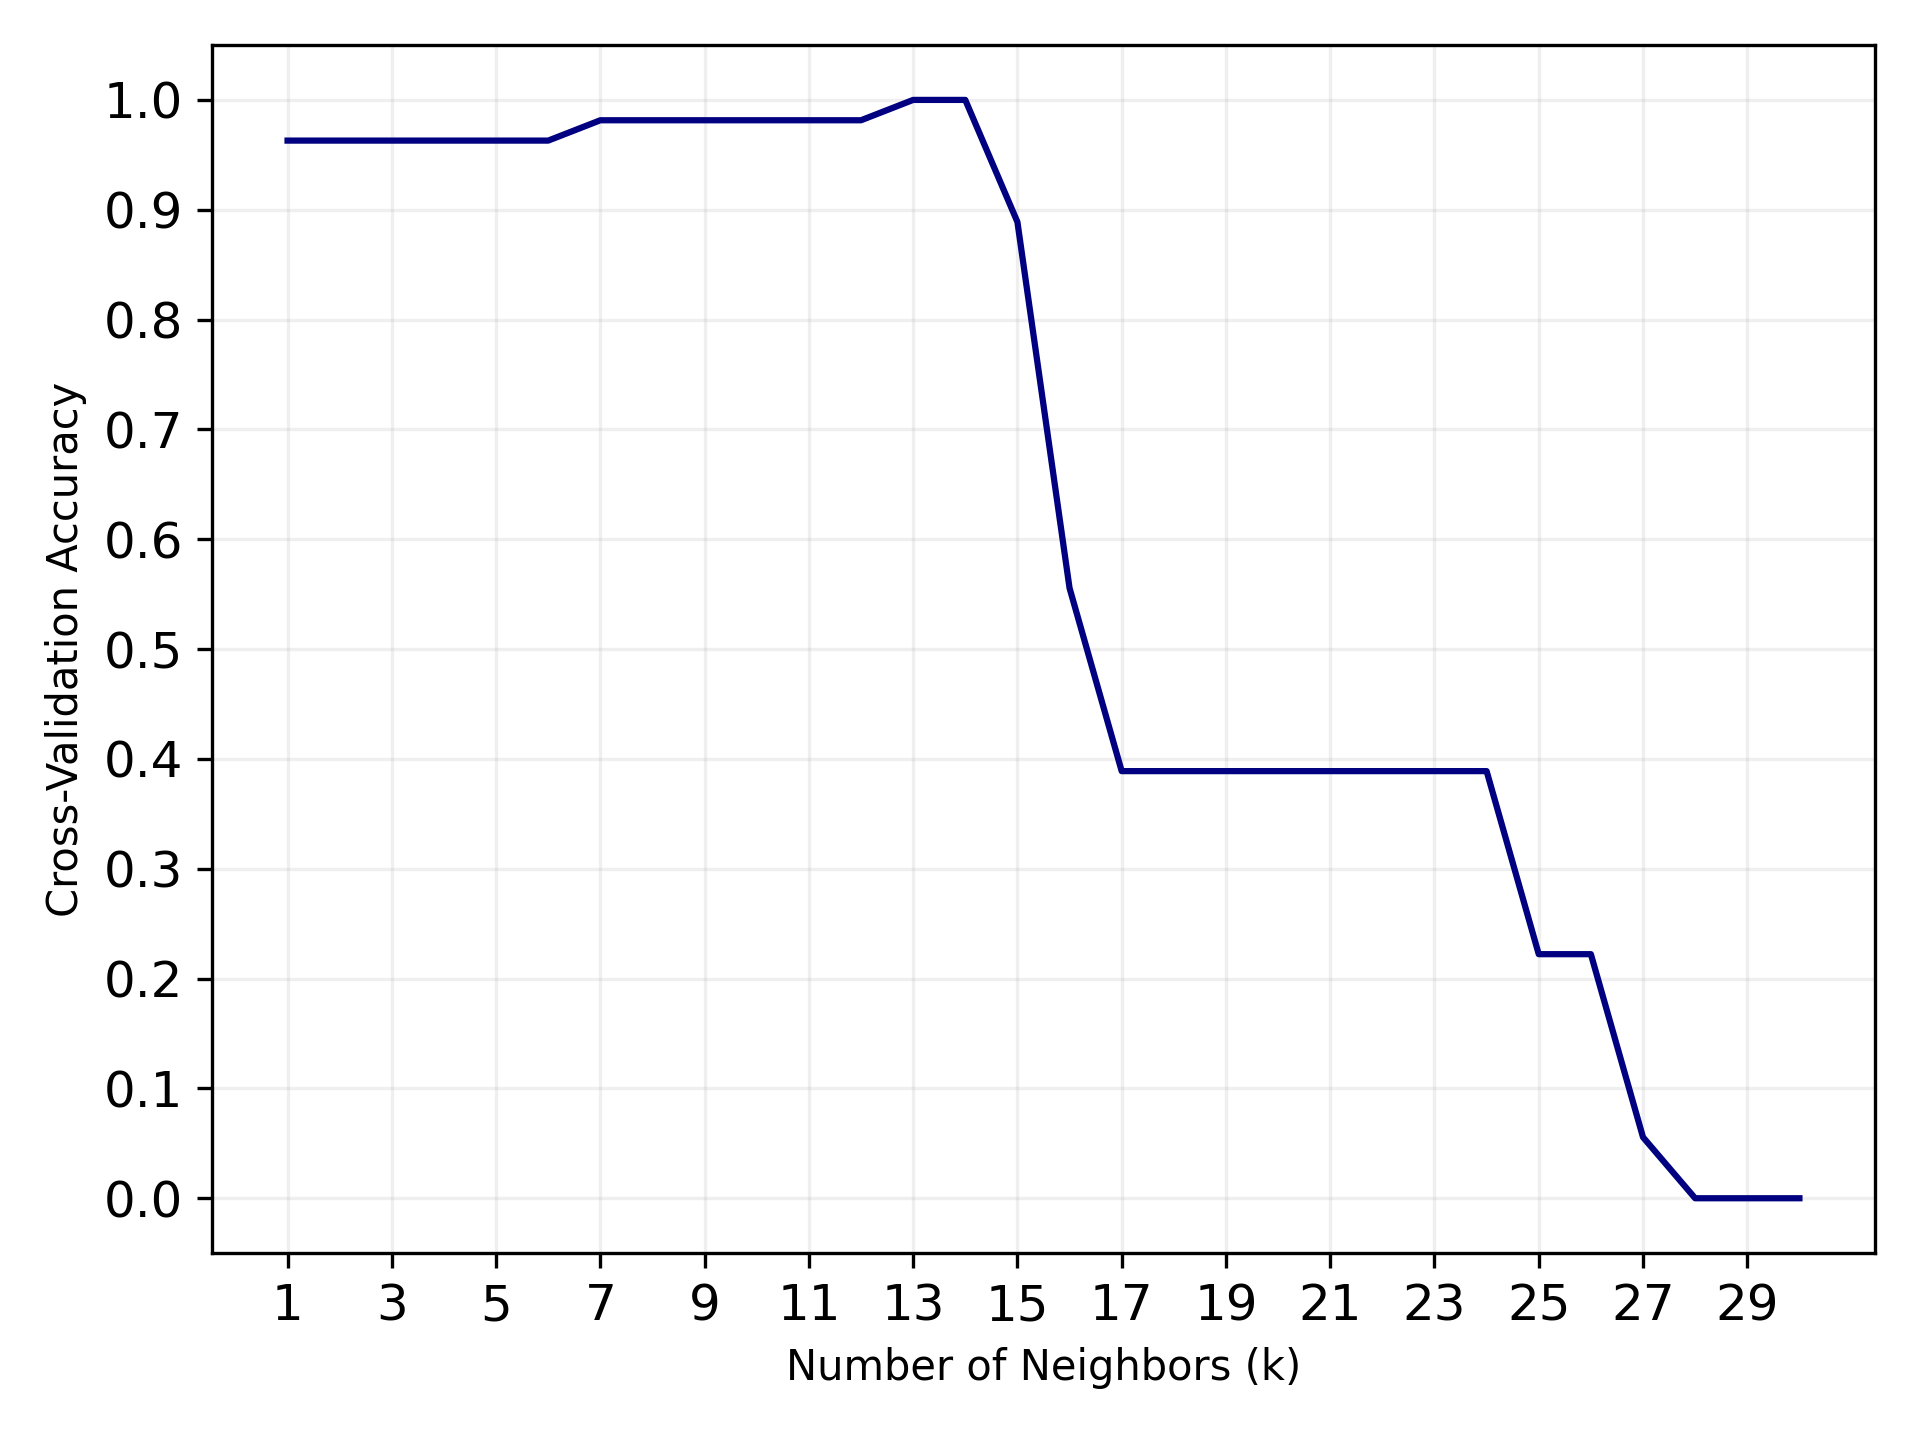
\includegraphics[width=0.5\linewidth]{figures/Letter_knn_accuracy_vs_k.png}
    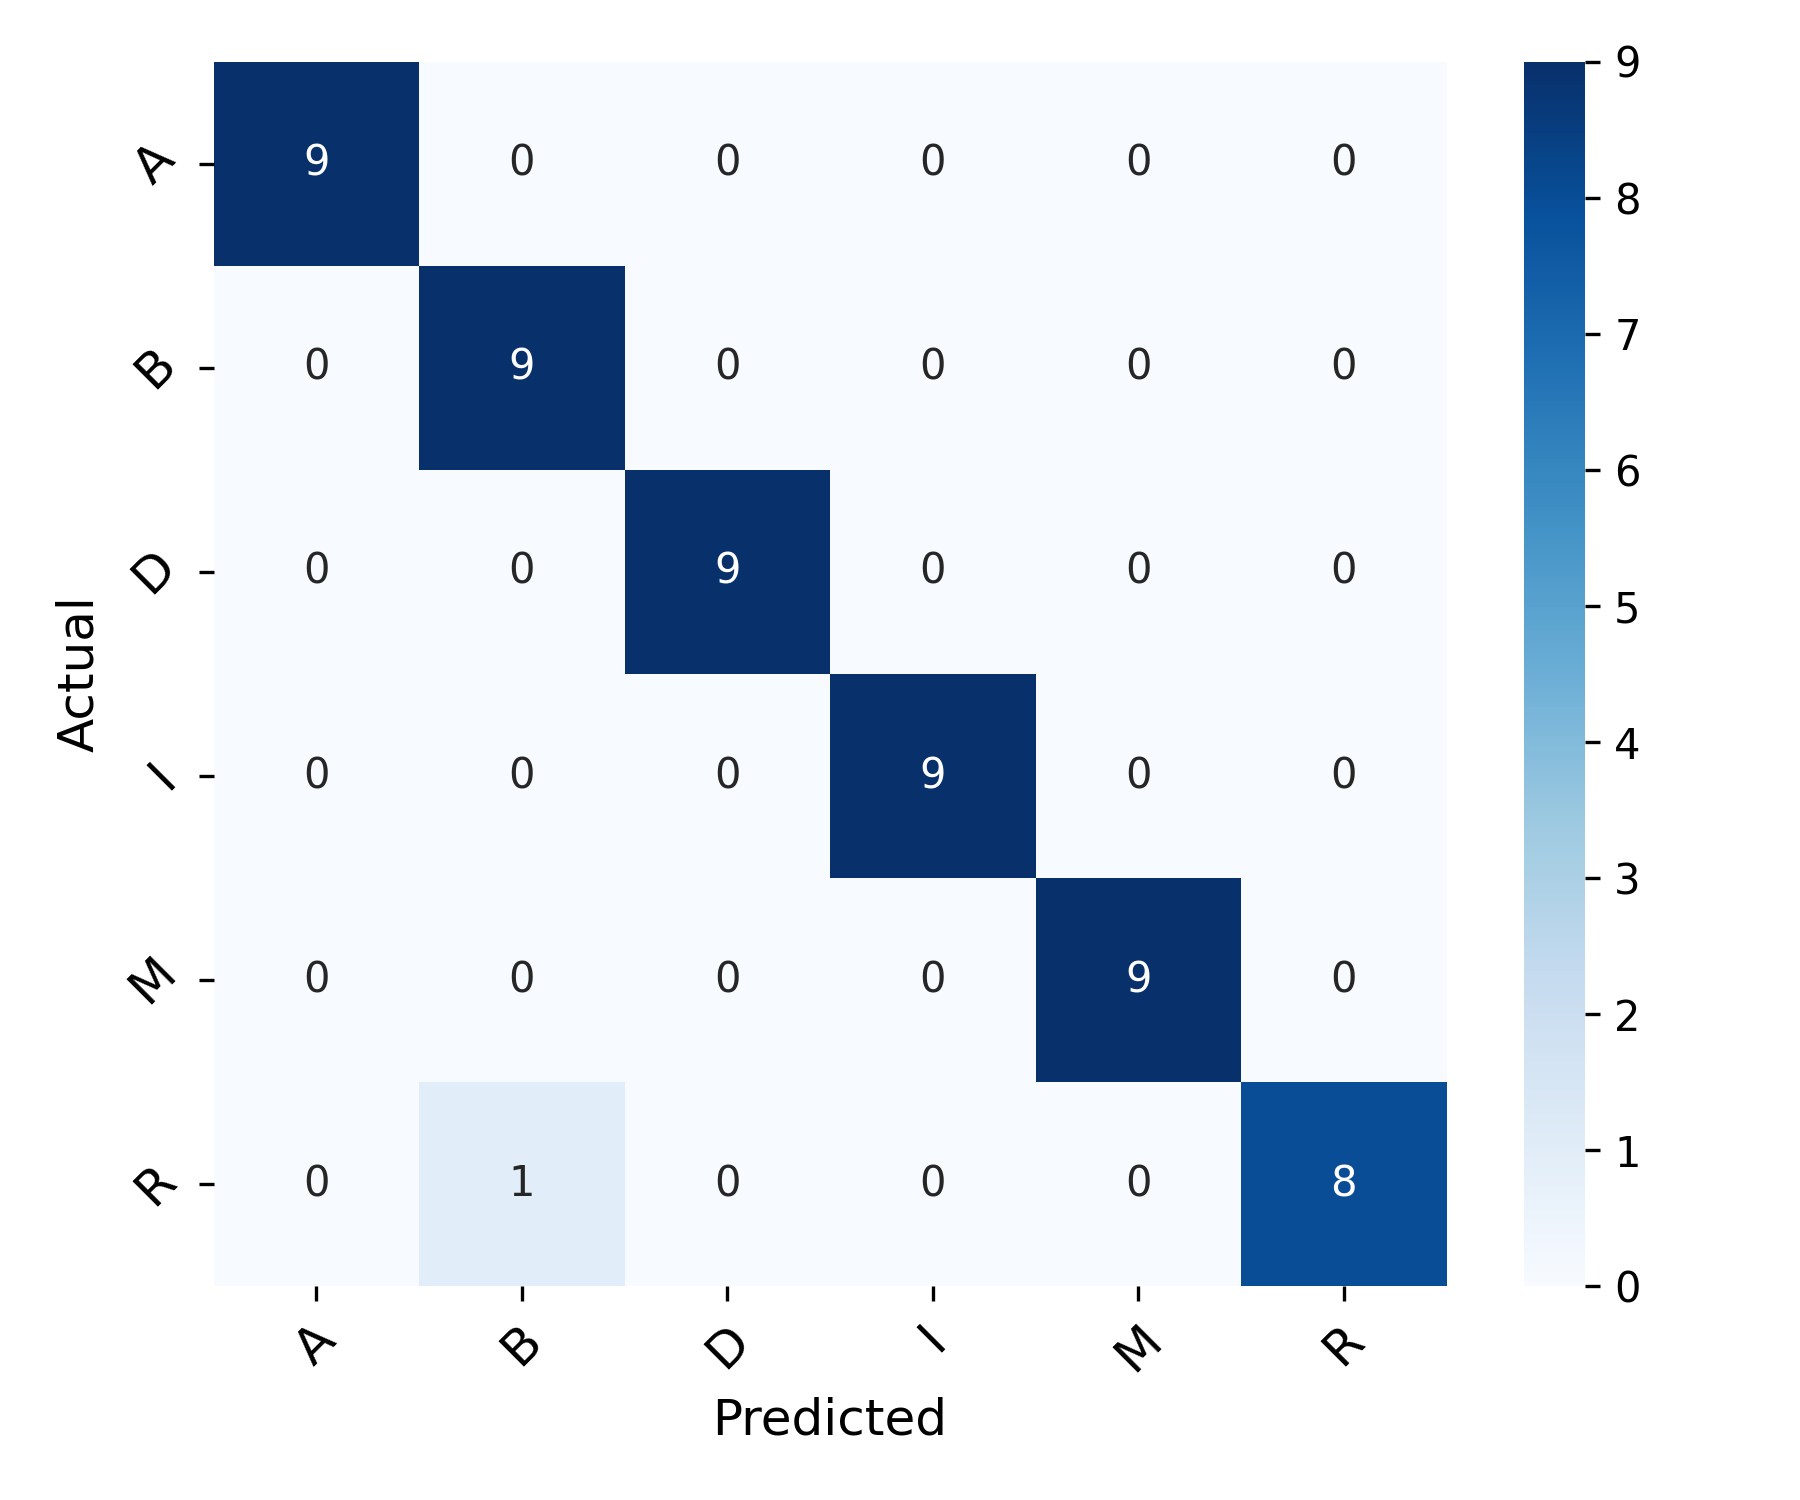
\includegraphics[width=0.45\textwidth]{figures/Letter_confusion_matrix.png}
    \caption{(Left) Accuracy of KNN classifier for different $k$ values during 5-fold cross-validation. The optimal $k = 9$ achieved $98.15\%$ accuracy.\\
    (Right) Confusion matrix showing how the actual classes match with the predicted class. Each $(i,j)$-th cell indicate number of times an image from category $i$ was classified as category $j$.}
    \label{fig:knn_accuracy_letter}
\end{figure}
The optimal value of $k$ is 9 (see \cref{fig:knn_accuracy_letter}), which yields $98.15\%$ accuracy.
We also performed leave-one-out cross-validation (LOO-CV), confirming the accuracy remains at $98.15\%$.
This shows the model is highly effective, though some misclassifications occur.
Like the MPEG-7 dataset, this letter dataset is quite small, with only nine point clouds in each of the six classes.
Expanding the experiment on a more robust dataset could improve the accuracy further.




%
%
%
%
These results further support the idea that the approximate interleaving distance captures meaningful topological variation in the data.

